In questo capitolo verrà trattata la fase di modellazione, che rappresenta la fase principale di ogni processo di sviluppo di un'applicazione.

Attraverso la modellazione è possibile definire un {\itshape modello di dominio}, il quale assume il compito di descrivere un ecosistema di entità del mondo reale che interagiscono tra loro, attraverso una rappresentazione grafica per mezzo di diagrammi.

Per poter apprendere i metodi di sviluppo di un modello di dominio vi è prima di tutto il bisogno di comprendere il concetto di Analisi Orientata agli Oggetti (OOA) e Progettazione Orientata agli Oggetti (OOP). Inoltre è di notevole aiuto conoscere i concetti base di UML, una notazione standard per la creazione di diagrammi.

\section{Analisi e Progettazione \\ Orientata agli Oggetti} % (fold)
\label{sec:analisi_orientata_agli_oggetti}

Prima ancora di definire il concetto di Analisi Orientata agli Oggetti vi è il bisogno di soffermarsi sul significato di analisi.
Come il termine stesso indica, l'analisi enfatizza un'investigazione del problema e dei requisiti in un universo di riferimento, anziché una soluzione. Nell'esempio di questo ambiente di studio, bisogna prima di tutto comprendere il funzionamento di un sistema di trasporti urbani e le sue proprietà.
Al contrario, la progettazione enfatizza una soluzione concettuale che soddisfa i requisiti, anziché la relavita implementazione. Infine il progetto può essere implementato, e l'implementazione (ovvero il codice) esprime il progetto realizzato vero e proprio.

Dunque nell'analisi orientata agli oggetti vi è un'enfasi sull'identificazione e la descrizione di oggetti, o di concetti, nel dominio del problema. Durante la progettazione orientata agli oggetti l'enfasi è sulla definizione di oggetti software e del modo in cui questi collaborano per soddisfare i requisiti.
% section analisi_orientata_agli_oggetti (end)

\section{UML (Unified Modeling Language)} % (fold)
\label{sec:uml_}

L'Unified Modeling Language, o UML, è un linguaggio di modellazione e specifica basato sul paradigma orientato agli oggetti. Esso rappresenta 
uno standard {\itshape de facto} per la notazione di diagrammi per disegnare o rappresentare figure relative al software, ed in particale relative al software OO.
UML consente di costruire modelli OO per rappresentare domini di diverso genere. Nel contesto dell'ingegneria software, viene utilizzato soprattutto per descrivere il dominio applicativo di un sistema software e/o il comportamento e la struttura del sistema stesso.
Il modello è strutturato secondo un insieme di viste che rappresentano diversi aspetti della cosa modellata, sia a scopo di analisi che di progetto, mantenendo la tracciabilità dei concetti impiegati nelle diverse viste. Oltre che per la modellazione dei sistemi software viene usato per descrivere domini di altri tipi, ad esempio sistemi hardware, sistemi di gestione o strutture organizzative in un'ecosistema specifico. 
% section uml_ (end)

\newpage

\section{Il modello di dominio} % (fold)
\label{sec:il_modello_di_dominio}

Il modello di dominio è la rappresentazione più importante e classica impiegata nell’analisi orientata agli oggetti. Esso illustra i concetti significativi di un dominio. Può fungere da sorgente di inspirazione per la progettazione di alcuni oggetti software.
La notazione di base è banale, ma per ottenere un modello utile è necessario seguire delle linee guida di modellazione molto sottili.
L’identificazione di un ricco insieme di classi concettuali è al centro dell’analisi orientata agli oggetti. Se viene effettuata con perizia e con un breve investimento di tempo solitamente ripaga nella progettazione.

Il passo essenziale dell’analisi orientata agli oggetti è la decomposizione di un dominio in concetti o oggetti significativi. 
Un modello di dominio è una rappresentazione visuale di classi concettuali o di oggetti del mondo reale di un dominio e non di oggetti software, è illustrato con un insieme di diagrammi delle classi in cui sono definite operazioni. Esso fornisce un punto di vista concettuale e mostra: 

\begin{itemize}
    \item Oggetti di dominio o classi concettuali
    \item Associazioni tra le classi concettuali
    \item Attributi di classi concettuali
\end{itemize}

Il modello mostra un’astrazione delle classi concettuali, poiché vi sono molte altre informazioni che si potrebbero comunicare in merito alle classi prese in esame. Le informazioni che esso rappresenta possono essere espresse, in alternativa, come semplice testo, ma l’uso di un linguaggio visuale permette di capire più facilmente i termini e soprattutto le relazioni tra di esse, poichè il cervello umano è bravo a comprendere elementi illustrati graficamente e linee di connessione.
Pertanto il modello di dominio è un dizionario visuale delle astrazioni significative, della terminologia del dominio e del contenuto informativo del sistema in esame.

Dunque ricapitolando, un modello di dominio è relativo a un punto di vista puramente concettuale e pertanto descrive oggetti del mondo reale e non da un punto di vista software.
Tuttavia a questo termine sono stati dati altri significati, come per indicare lo strato degli oggetti sodtware di un dominio, ovvero lo strato degli oggetti software sotto lo strato di presentazione o interfaccia.
La definizione corretta non esiste, o meglio ogni definizione è a suo modo corretta, a seconda di ciò che si vuole rappresentare. Può capitare dunque di fare confusione quando si vuol parlare  di modello di dominio, dunque si indicherà come strato di dominio il secondo significato del modello, quello orientato agli oggetti software, come avviene nella maggior parte dei casi.

\subsection{Classi concettuali} % (fold)
\label{sub:classi_concettuali}

% subsection subsection_name (end)
Una classe concettuale, secondo una definizione informale, è un’idea, una cosa o un’oggetto. Più formalmente una classe concettuale può essere considerata in termini del suo simbolo, della sua intensione ed estensione:
\begin{itemize}
    \item Simbolo: parole o immagini che rappresentano una classe concettuale
    \item Intensione: la definizione di una classe concettuale
    \item Estensione: l'insieme di esempi a cui la classe concettuale si applica
\end{itemize}
Ad esempio nel caso d’interesse di questo trattato, si può assegnare un nome ad una classe concettuale in base al simbolo Fermata.
L’intensione di una fermata può affermare che essa rappresenta il luogo ove è collocato un punto per la salita e discesa dei passeggeri su un autobus, e pertanto avrà un nome che la distingue nel percorso e una posizione che ne permette la locazione.
L’estensione di Fermata sono tutti gli esempi di fermate. In altre parole, l’insieme di tutti i punti di fermata lungo un percorso preso in esame.

\begin{figure}[htbp]
\begin{center}
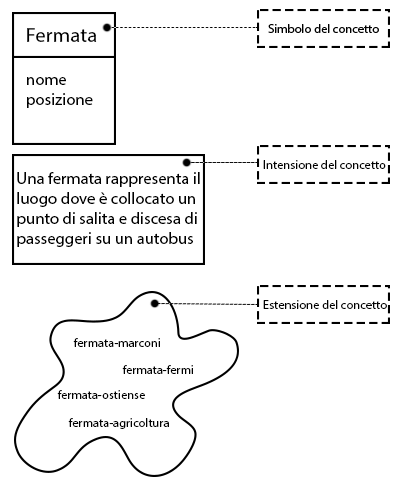
\includegraphics{contents/images/esempio_fermata}
\end{center}
\caption{Classe concettuale di Fermata}
\label{fig:fermata}
\end{figure}
% section il_modello_di_dominio (end)

\newpage

\subsection{Perché creare il modello} % (fold)
\label{sub:perch_creare_il_modello}

Il processo di concepimento del modello di dominio  di un caso di studio è un’attività largamente utilizzata nel mondo dello sviluppo software, questo perché permette di ottenere un salto rappresentazionale basso nella modellazione orientata agli oggetti.
Questo è un’idea fondamentale nel paradigma OO: utilizzare nomi di classi software nello strato del dominio ispirati ai nomi del modello di dominio, con oggetti dotati di informazioni e responsabilità aventi attinenza con il dominio.
Questo processo permette una trasformazione graduale del caso di studio, riplasmando gli oggetti del mondo reale in entità via via sempre più astratte ed adatte all’ambiente di programmazione.
Ciò comporta un risparmio in termini di tempo e denaro, rendendo l’attività di sviluppo software più facile ed efficiente.
% subsection perch_creare_il_modello (end)

\newpage

\subsection{Come creare il modello} % (fold)
\label{sub:come_creare_il_modello}

Nella creazione di un modello di dominio vengono effettuati tre passi principali: identificare le classi concettuali; disegnarle all’interno di un diagramma UML; aggiungere dunque le relative associazioni ed attributi.

Per svolgere il primo passo esistono varie strategie. Quella utilizzata in questo elaborato è una strategia semplice ma efficace: descrivendo il processo di funzionamento dell’ecosistema preso in esame, possono essere distinti elementi e termini chiave che diverranno candidati a possibili classi concettuali.

Si ha però bisogno di fare particolare attenzione nello svolgimento di questo approccio: in quanto il suo punto debole è l’imprecisione del linguaggio naturale. Ad esempio un possibile caso di ambiguità risiede nell’avere più locuzioni nominali che possono rappresentare la stessa classe concettuale o attributo.
% subsection come_creare_il_modello (end)

\subsubsection{Scelta delle classi} % (fold)
\label{ssub:scelta_delle_classi}

Nella scelta dei nomi delle classi concettuali è sempre preferibile utilizzare i nomi esistenti nel territorio, cercando di specificarne il più possibile il suo ruolo, così da facilitare la comprensione dellpambiente in fase di progetto. Vengono inoltre escluse tutte le caratteristiche irrilevanti o non essenziali, oltre che ovviamente evitare di aggiungere elementi che non esistono nell’ambiente di studio, per manentere il modello il più snello ed essenziale possibile.

Un errore comune nella scelta delle classi è quello di concepire una potenziale classe come attributo di un’altra. La regola utilizzata per ovviare a questo problema è quella di pensare agli elementi nel mondo reale: se esse non vengono immediatamente distinte come semplici numeri o descrizioni, allora  non rappresentano degli attributi ma probabilmente delle classi concettuali.

Durante la scelta delle classi, è utile trovare e mostrare associazioni necessarie per soddisfare i requisiti informativi degli scenari correnti in corso di sviluppo, nonché quelle che contribuiscono alla comprensione del dominio.
Un'associazione è quindi definita come una relazione tra classi, la quale indica una connessione significativa e interessante.

Le associazioni che è utile mostrare sono solitamente quelle che implicano la conoscenza di una relazione che deve essere memorizzata per un certo periodo che, a seconda del contesto, potrebbe essere di millisecondi o addirittura anni.
Poiché il modello di dominio descrive un punto di vista concettuale, queste affermazioni sulla necessità di ricordare fanno riferimento ad una necessità nel mondo reale, e non nell'ambiente di rappresentazione software, anche se durante l'implementazione ci si imbatterà a dover soddisfare molte necessità simili.
E' sempre un bene però evitare di inserire troppe associazioni in un modello di dominio perché, come detto in precedenza, avere un modello che sia semplice e snello facilita la comprensione in fase di sviluppo e garantisce una concezione più veloce ed intuitiva. Dunque è sempre opportuno decidere con attenzione e parsimonia le associazioni, concentrandosi solamente su ciò che si deve memorizzare.
% subsubsection scelta_delle_classi (end)

\subsection{Associazioni} % (fold)
\label{sub:associazioni}

Nel diagramma, un'associazione è rappresentata come una linea che collega le classi partecipanti alla relazione. Le estremità di un'associazione possono contenere un'espressione di molteplicità, la quale indica le relazioni numeriche tra le istanze delle classi.
Ogni associazione è per natura bidirezionale, nel senso che è possibile una navigazione logica dalle istanze di una delle due classi a quelle dell'altra, e viceversa. Ma questa navigazione è puramente astratta, essa non è un'affermazione su connessioni tra entità software.
La molteplicità dell'associazione definisce quante istanze di una classe possono essere associate ad un'istanza di un'altra classe relazionata con la prima.
Un esempio calzante in questo trattato è quello dell'associazione tra Direzione e Fermata: ogni direzione di una linea di trasporti è composta da una discreta quantità di fermate, mentre una fermata può appartenere ad una o più direzioni, dunque l'associazione tra queste due classi è N a N.

Infine, si assegna ad ogni associazione un nome rappresentato come una locuzione verbale, così da facilitare la comprensione del ruolo della relazione tra le due classi. Si ricordi che un'associazione è leggibile in entrambe le direzioni, per cui anche se il nome induce alla lettura in un senso unico, esso può essere comunque ``ribaltato'' per garantirne la lettura nell'altro verso.
% subsection associazioni (end)

\subsection{Attributi} % (fold)
\label{sub:attributi_mod}

Per quanto riguarda gli attributi, essi definiscono un valore logico, in altre parole un dato, di un oggetto. E' utile identificare gli attributi delle classi concettuali, cosi da soddisfare i contenuti informativi per gli scenari correnti nel corso dello sviluppo.
Gli attributi vengono scelti attraverso i casi d'uso, quando i requisiti suggeriscono una necessità di ricordare informazioni. Nel diagramma, essi sono collocati all'interno delle classi concettuali a cui fanno riferimento rappresentati attraverso il loro nome.
% subsection attributi (end)

\section{Il MDD della rete trasporti pubblici} % (fold)
\label{sec:il_MDD_della_rete_trasporti_pubblici}

Avendo dunque specificato la struttura e la costruzione del modello di dominio, si procede ora alla realizzazione del modello specifico all'ambiente preso in esame in questa tesi: la rete dei trasporti pubblici urbani.

Come si è già accennato in precedenza, una rete di trasporti pubblici di notevoli dimensioni comporta una ramificazione dei trasporti attraverso un'agglomerato di linee, le quali sono a loro volta suddivise in più direzioni per poter definire i percorsi che quella linea copre.
A sua volta, ogni direzione elenca un numero di fermate in cui è possibile attendere il passaggio dei vari mezzi di trasporto. Infine la rete di trasporti è composta dai mezzi stessi, come gli autobus, ai quali sarà definito un tragitto da percorrere a seconda della direzione a cui sono assegnati.
\newpage
Dunque si definisce ora un possibile caso d'uso d'interesse:
\begin{enumerate}
   \item un {\bfseries utente} consulta un'elenco di {\bfseries linee} per scegliere quella d'interesse
   \item l'{\bfseries utente} sceglie una {\bfseries direzione} di preferenza appartenente alla linea selezionata
   \item dunque consulta l'elenco di {\bfseries fermate} del tracciato preso in esame
   \item l'{\bfseries utente} sceglie dunque la {\bfseries fermata} in base alla sua {\bfseries posizione}
   \item l'{\bfseries utente} consulta dunque gli {\bfseries autobus} in arrivo
\end{enumerate}

Dall'elenco dell'analisi dei nomi e delle locuzioni nominali è possibile generare un elenco delle classi concettuali candidate per il dominio. Dal momento che si tratta di un sistema di trasporti pubblici, si pone l'attenzione prima di tutto sulle categorie che enfatizzano oggetti fisici e le relazioni tra di essi.
Come già visto da alcuni esempi precedenti, si possono individuare alcune classi principali di rilievo:

{\itshape Linea}

{\itshape Direzione}

{\itshape Fermata}

{\itshape Autobus}

In questo caso d'uso potrebbe essere preso in considerazione anche l'elemento Utente, ma al fine di questo progetto - il quale mira esclusivamente al monitoraggio dei trasporti pubblici e non ai servizi offerti al pubblico - questa classe concettuale non è di rilevanza, e verrà perciò scartata.
Dunque le classi concettuali del modello di dominio sono le seguenti:

\begin{figure}[htbp]
\begin{center}
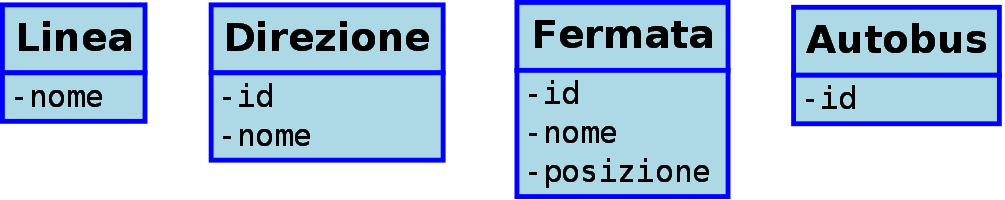
\includegraphics[width=10cm]{contents/images/classi_concettuali}
\end{center}
\caption{Classi concettuali}
\label{fig:classes}
\end{figure}

\newpage
Per ogni classe sono stati definiti anche i corrispettivi attributi d'interesse.

Nel caso della Linea, l'unico dettaglio di cui tenere traccia è il nome, che identifica univocamente la linea nell'insieme globale. Per quanto riguarda la direzione, essa è costituita da un nome di riferimento (usato solo per la consultazione) ed un ID, che ne permette la catalogazione.
Nel caso di Fermata, si può notare l'attributo nome, l'ID e la posizione ove la fermata è collocata, gestita attraverso una coordinata.
Per l'elemento Autobus, l'unico attributo di rilevanza è un ID, il quela permette di identificare un autobus in un vasto insieme di trasporti.

A questo punto si prosegue attraverso la concezione delle relazioni e la creazione delle associazioni tra classi.
Seguendo sempre il caso d'uso descritto in precedenza, una linea contiene un elenco di direzioni, mentre ogni direzione appartiene ad una e una sola linea. Viene quindi creata l'associazione ``Costituita da'' tra Linea e Direzione con molteplicità 1 a N.
Proseguendo, si può notare come a sua volta ogni direzione sia composta da un cospicuo numero di fermate, mentre una fermata può essere un punto di scambio tra più direzioni. Dunque l'associazione ``Composta da'' tra Direzione e Fermata avrà molteplicità N a N.
Concludendo con l'ultima classe, un autobus è associato ad'una direzione univoca e, durante il suo tragitto, si ferma in ogni fermata definita dalla direzione. In una direzione transitano più autobus e, allo stesso modo, in una fermata possono fermare più autobus. Le relazioni tra Autobus e Direzione e Autobus e Fermata saranno definite rispettivamente dall'associazione ``Appartiene'' di molteplicità N a 1 e dall'associazione `Collocato su'' di molteplicità N a 1.
\newpage
Avendo quindi specificato tutte le associazioni essenziali, il diagramma del modello di dominio assume questa forma:

\begin{figure}[htbp]
\begin{center}
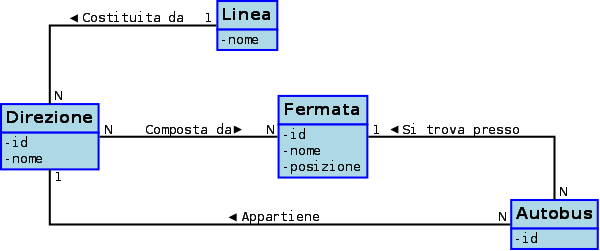
\includegraphics[width=10cm]{contents/images/modelloDominio}
\end{center}
\caption{Classi concettuali}
\label{fig:domain_model}
\end{figure}

La rappresentazione finale del modello di dominio di questo caso di studio è un diagramma molto semplice e snello, racchiudendo solamente i dettagli essenziali per la progettazione del servizio descritto in questo elaborato.
Come già spiegato in precedenza, il suo scopo non è descrivere in maniera esaustiva il comportamento di un servizio di trasporti urbani, ma si limita a definirne una concezione semplificata e, allo stesso tempo, sufficientemente completa per poter progettare un servizio efficiente.

Nel capitolo seguente si farà riferimento a questo modello di dominio per la definizione del {\itshape diagramma delle classi di progetto}, il quale si assumerà il compito di adattare la visione del modello ad un punto di vista software.
% section il_modello_della_rete_trasporti_pubblici (end)

\newpage